\documentclass{beamer}
\usepackage[utf8]{inputenc}
\usepackage{tikz}
\usepackage{xcolor}
\usetikzlibrary{positioning}
\usetheme{metropolis}           % Use metropolis theme
\title{Dipartimento di Ingegneria dell'Informazione}
\date{\today}
\author{}
\institute{Università degli Studi di Padova}
\begin{document}
	\begin{frame}
		\maketitle
		\begin{tikzpicture}[overlay, remember picture]
		% \node[above right=1cm and .8cm of current page.south west] {
\includegraphics[width=2cm]{logo.png}};
		% \node[above =1cm of current page.south] {
\includegraphics[width=2cm]{logo.png}};
		\node[above left=1cm and .8cm of current page.south east] {
\includegraphics[width=2cm]{logo.png}};
		\end{tikzpicture}
	\end{frame}
  \section{Quanti anni devo studiare?}
  \begin{frame}{Corso di studi}
    \centering
		\begin{figure}
  		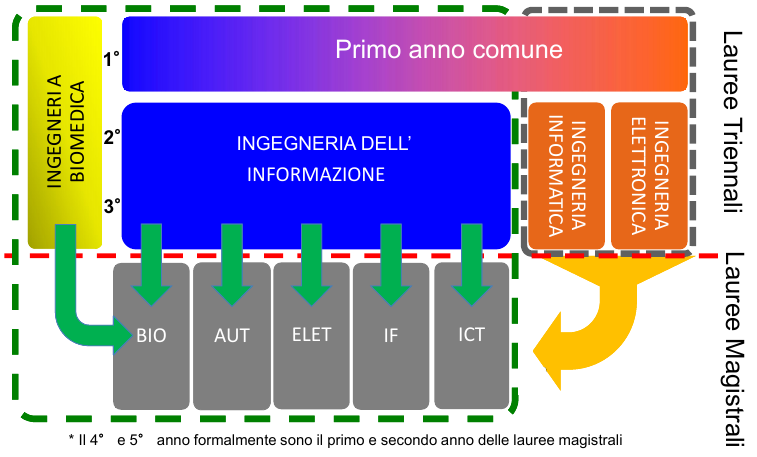
\includegraphics[width=10cm]{percorso.png}
  	\end{figure}
  \end{frame}
	\section{Come faccio a laurearmi?}
	\begin{frame}{Crediti Formativi (CFU)}
		Ogni anno è necessario conseguire circa 60 crediti formativi, per un totale di \textbf{180 CFU in triennale} e \textbf{120 CFU in magistrale}.

		Dopo aver passato un esame si \textit{guadagnano} alcuni punti CFU, \textbf{in linea generale} più un esame è grosso e difficile più CFU fa \textit{guadagnare}.
	\end{frame}
	\begin{frame}{Crediti Formativi (CFU)}
		\centering
		\textbf{1 CFU $\leftrightarrow$ 25 ore di lavoro}

		\textbf{1 CFU $\leftrightarrow$ 8 ore di lezione e 17 di studio individuale}
	\end{frame}
	\section{Cosa studio a Ingegneria dell'Informazione?}
	\begin{frame}{Primo anno}
		\begin{itemize}
			\setlength\itemsep{1em}
			\item[ ] {\color{red}Analisi Matematica 1 (12)}
			\item[ ] {\color{blue}Fondamenti di Informatica (9)}
			\item[ ] {\color{red}Algebra Lineare e Geometria (12)}
			\item[ ] {\color{red}Fisica Generale 1 (12)}
			\item[ ] {\color{blue}Architettura degli Elaboratori (9)}
		\end{itemize}
	\end{frame}
	\begin{frame}{Secondo anno}
		\begin{itemize}
			\setlength\itemsep{1em}
			\item[ ] {\color{red}Analisi Matematica 2 (12)}
			\item[ ] {\color{red}Fisica Generale 2 (9)}
			\item[ ] {\color{blue}Dati e Algoritmi 1 (9)}
			\item[ ] {\color{blue}Analisi dei Dati (9)}
			\item[ ] {\color{blue}Campi elettromagnetici e propagazione (6)}
			\item[ ] {\color{blue}Elettrotecnica (6)}
			\item[ ] {\color{blue}Segnali e Sistemi (9)}
		\end{itemize}
	\end{frame}
	\begin{frame}{Terzo anno}
		\begin{itemize}
			\setlength\itemsep{1em}
			\item[ ] {\color{blue}Controlli Automatici (9)}
			\item[ ] {\color{blue}Elettronica (9)}
			\item[ ] {\color{blue}Sistemi e Modelli (9)}
			\item[ ] {\color{blue}Algoritmi per l'ingegneria (6)}
			\item[ ] {\color{blue}Elettronica digitale (6)}
			\item[ ] {\color{blue}Telecomunicazioni (9)}
			\item[ ] {\color{blue}Corsi a scelta (12)}
		\end{itemize}
	\end{frame}
	\begin{frame}{Corsi a scelta (12 CFU)}
		\begin{itemize}
			\setlength\itemsep{0.5em}
			\item[ ] {\color{blue}Laboratorio di Internet and Multimedia (6)}
			\item[ ] {\color{blue}Laboratorio di Ottica per l'Ingegneria dell'Informazione (6)}
			\item[ ] {\color{blue}Laboratorio di Segnali e Misure (6)}
			\item[ ] {\color{blue}Project Management (6)}
			\item[ ] {\color{blue}Storia della tecnologia dell'informazione (6)}
			\item[ ] {\color{blue}Laboratorio di Automatica (6)}
			\item[ ] {\color{blue}Laboratorio di Bioingegneria (6)}
			\item[ ] {\color{blue}Laboratorio di Ingegneria Informatica (6)}
			\item[ ] {\color{blue}Laboratorio Microelettronica (6)}
		\end{itemize}
	\end{frame}
	\begin{frame}
		\begin{description}
			\setlength\itemsep{1em}
			\item[Laurea Triennale in Ingegneria Biomedica] http://didattica.unipd.it/off/2016/LT/IN/IN0512
			\item[Laurea Triennale in Ingegneria Informatica] http://didattica.unipd.it/off/2017/LT/IN/IN0508
			\item[Laurea Triennale in Ingegneria Elettronica] http://didattica.unipd.it/off/2017/LT/IN/IN0507
		\end{description}
	\end{frame}
	\section{E dopo la triennale?}
	\begin{frame}{Lauree Magistrali}
		\textbf{
			\begin{itemize}
				\setlength\itemsep{1em}
				\item[ ] Ingegneria Informatica
				\item[ ] Ingegneria Elettronica
				\item[ ] Ingegneria dell'Automazione
				\item[ ] Bioingegneria
				\item[ ] ICT for Internet and Multimedia
				\item[ ] {\color{gray}Laurea magistrale in un'altra università italiana o all'estero!}
			\end{itemize}
		}
	\end{frame}
	\begin{frame}{LM in Ingegneria Informatica}
		\begin{columns}
			\begin{column}{0.4\textwidth}
				\centering
				
\includegraphics[width=0.6\textwidth]{big_data.png}

				Big Data

				\vspace{0.5cm}
				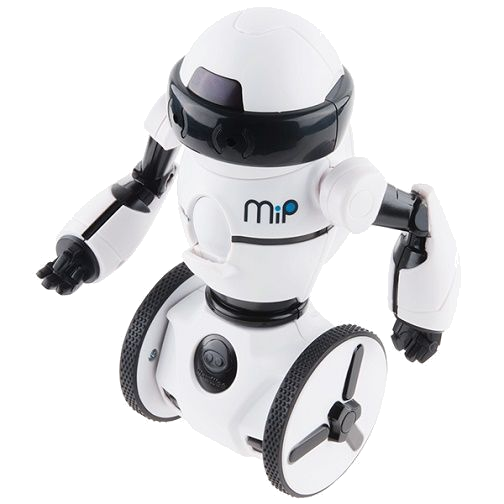
\includegraphics[width=0.6\textwidth]{robotica_inf.png}

				Robotica e Intelligenza Artificiale
			\end{column}
			\begin{column}{0.4\textwidth}
				\centering
				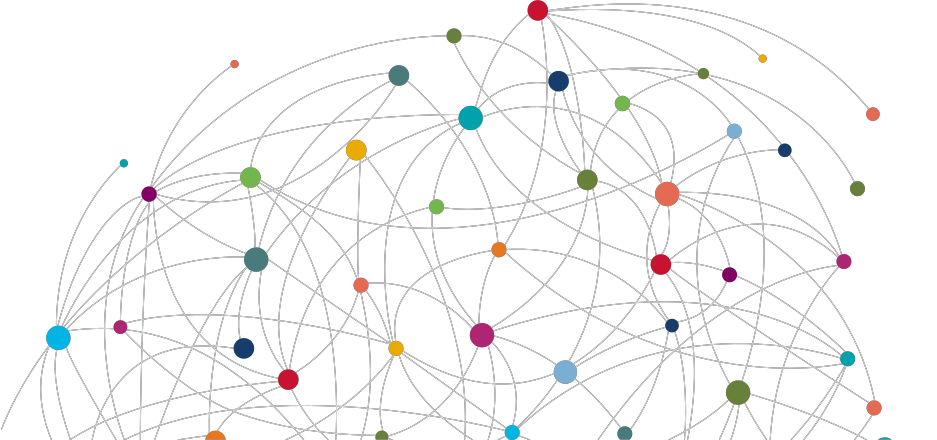
\includegraphics[width=0.8\textwidth]{network.png}

				Reti sociali, di calcolatori e IoT

				\vspace{0.5cm}
				
\includegraphics[width=\textwidth]{sistemi-operativi.png}

				Sistemi Operativi
			\end{column}
		\end{columns}
	\end{frame}
\end{document}
